\section{Results}

\begin{table}[htbp]
\footnotesize
\centering
\caption{Thrombectomy use and arrival times by stroke type, direct admission (to MT-capable centre) status, and year}
\label{tab:thrombectomy}
\begin{tabular}{l  l l r r r r r }
\hline
\textbf{Stroke type} &
\makecell{\textbf{Direct}\\\textbf{admission}} &
\textbf{Year} &
\makecell{\textbf{MT use}\\\textbf{\%)}} &
\makecell{\textbf{\# MT}\\\textbf{performed}} &
\makecell{\textbf{Patient}\\\textbf{count}} &
\makecell{\textbf{Arrival to MT}\\\textbf{mean (mins)}} &
\makecell{\textbf{Arrival to MT}\\\textbf{median (mins)}} \\
\hline
All admissions & No & 2023 & 3.03 & 1692 & 55775 & 301 & 239 \\
 &  & 2024 & 3.72 & 2092 & 56,297 & 309 & 234 \\
 &  & 2025 & 4.08 & 2297 & 56,257 & 301 & 227 \\
 &  & All & 3.72 & 6081 & 168,329 & 304 & 233 \\
\cline{2-8}
 & Yes & 2023 & 5.78 & 1323 & 22,887 & 177.39 & 121 \\
 &  & 2024 & 6.15 & 1363 & 221,63 & 207 & 139 \\
 &  & 2025 & 6.78 & 1501 & 22,142 & 262 & 132 \\
 &  & All & 6.15 & 4187 & 67,192 & 217.04 & 131 \\
\hline
Non-mild ischaemic & No & 2023 & 8.50 & 1614 & 18,988 & 292 & 236 \\
 (NIHSS $>$ 5 or LVO) &  & 2024 & 10.47 & 2018 & 19,268 & 300 & 232 \\
 &  & 2025 & 12.05 & 2277 & 18,904 & 298 & 225 \\
 &  & All & 10.34 & 5909 & 57,160 & 297 & 230 \\
 \cline{2-8}
 & Yes & 2023 & 14.63 & 1222 & 8,354 & 166 & 118 \\
 &  & 2024 & 15.73 & 1302 & 8,277 & 195 & 136 \\
 &  & 2025 & 17.99 & 1481 & 8,231 & 254 & 131 \\
 &  & All & 16.11 & 4005 & 24,862 & 208 & 129 \\
\hline
\end{tabular}
\end{table}

\begin{figure}
    \centering
    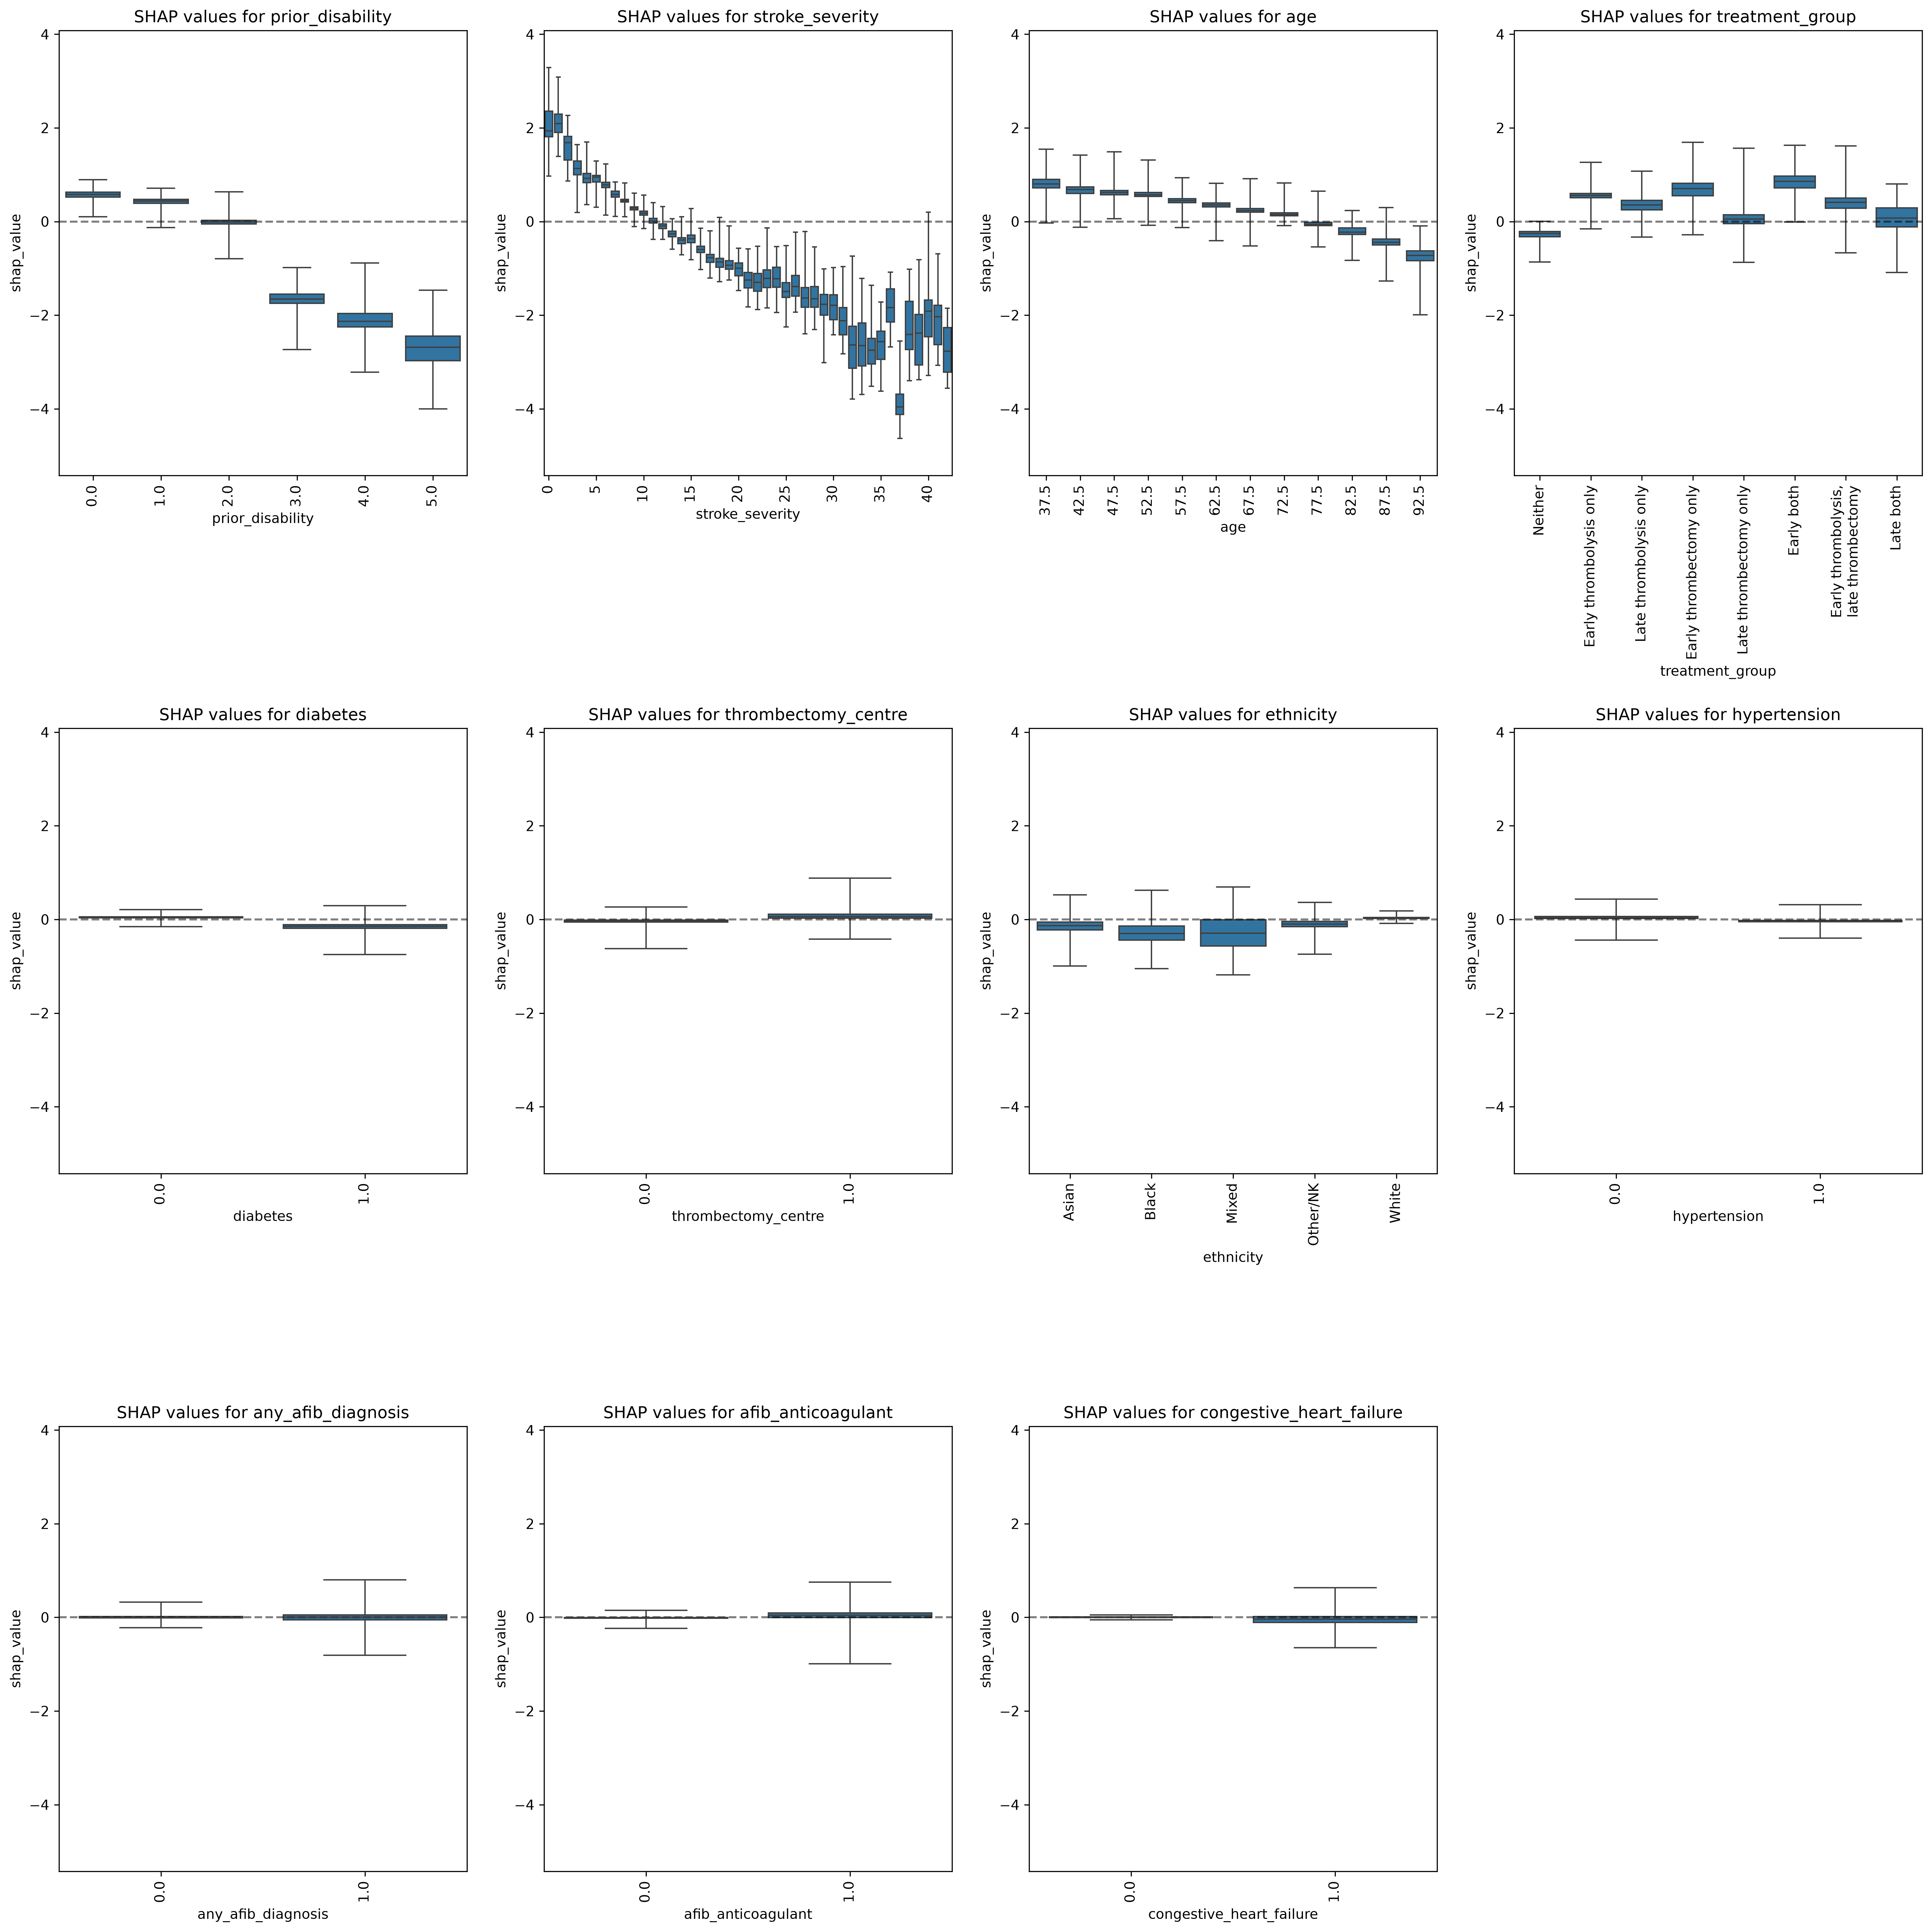
\includegraphics[width=1\linewidth]{images/01b_all_non_mild_mrs_2_shap_box_plots_outcome.png}
    \caption{Feature-specific distributions of SHAP values for functional independence following stroke. Box plots show Shapley additive explanation (SHAP) values for each predictor level or category from the fitted prediction model, expressed on the log-odds scale for discharge with a modified Rankin Scale (mRS) score of 0–2. Positive SHAP values indicate that a feature value increased the model-predicted odds of functional independence relative to the model’s baseline prediction, whereas negative values indicate decreased predicted odds. The final log odds of being discharged mRS 0-2 is the sum of all SHAP values for any individual patient and a common baseline SHAP value for all patients (0.854). The dashed horizontal line denotes no contribution to the log odds. Boxes represent the interquartile range, central lines the median, and whiskers the dispersion of SHAP values.}
    \label{fig:main_shap_mrs2}
\end{figure}



\begingroup
\footnotesize
\begin{longtable}[]{@{}lllll@{}}
\caption{Target trial emulation, matching (with \textit{k nearest neighbours}) patients who received thrombectomy after transfer from an IVT-only centre to those who received thrombectomy after being admitted directly to a thrombectomy-capable centre. *** P $<$ 0.001, t-test or Chi\textsuperscript{2} test as appropriate.}\\
\toprule
& \multicolumn{2}{c}{\textbf{Thrombectomy after transfer from}} & \multicolumn{2}{c}{\textbf{Thrombectomy after direct admission}} \\
& \multicolumn{2}{c}{\textbf{an IVT centre (n=3,678)}} & \multicolumn{2}{c}{\textbf{to a MT centre (n=3,678)}} \\
\textbf{Feature} & \textbf{Mean} & \textbf{SD} & \textbf{Mean} & \textbf{SD} \\
\midrule
\endhead
\bottomrule
\endlastfoot
\textit{Features matched on:} \\
Age (based on 5-year bands) & 70.5 & 13.7 & 70.3 & 13.9 \\
Stroke severity & 16.1 & 6.1 & 16.1 & 6.3 \\
Prior disability & 0.64 & 0.86 & 0.64 & 0.87 \\
Afib diagnosis & 0.34 & NA & 0.34 & NA \\
Afib anticoagulant & 0.20 & NA & 0.20 & NA \\
Onset known & 0.90 & NA & 0.90 & NA \\
Early (6hr) onset-to-arrival & 0.44 & NA & 0.44 & NA \\
Thrombolysis use & 0.44 & NA & 0.44 & NA \\
\midrule
\textit{Features included for descriptive statistics:}\\
Thrombectomy use & 1.00 & NA & 1.00 & NA \\
Arrival to thrombolysis time (mins) & 58 & 37 & 52\textsuperscript{***} & 32 \\
Arrival to thrombectomy time (mins) & 293 & 223 & 209\textsuperscript{***} & 1011 \\
\midrule
\textit{Outcome:}\\
Discharge disability (mRS) & 3.30 & 1.66 & 3.08\textsuperscript{***} & 1.73 \\
Discharged mRS 0-2 & 0.32 & NA & 0.39\textsuperscript{***} & NA \\
\end{longtable}
\endgroup

